\documentclass[
version=last,toc=bib,toc=graduated,toc=index,toc=listof,9pt,openany]{scrbook}
\pdfminorversion=4
\usepackage[utf8]{inputenc}
\usepackage{dejavu}

\usepackage{geometry}
\geometry{%a6paper
paperwidth=125mm, paperheight=168mm, 
portrait,
top=22mm, inner=22mm, outer=20mm, bottom=25mm,
headsep=3mm, footskip=12mm
}

\pdfminorversion=4


\usepackage[babel,german=quotes]{csquotes}
\usepackage{relsize}

\clubpenalty=10000 %keine Schusterjungen
 \widowpenalty=10000 
 \displaywidowpenalty=10000 % keine Hurenkinder

\usepackage[letterspace=16]{microtype} %schönerer Textsatz

\usepackage{graphicx} %Bilder

%Dateipfade, wo die Bilder liegen
\graphicspath{{images_print/}{icons/}{extra-pages/}}


\usepackage{tabu}
\usepackage{tabularx}
\usepackage{longtable}
\usepackage[table]{xcolor}
\usepackage{colortbl}

% PDF-Seiten einbinden
% pdfpages, darf erst nach colortbl geladen werden!
\usepackage{pdfpages}

% PDFs als Hintergrundbilder
% wallpaper, darf erst nach colortbl geladen werden!
\usepackage{wallpaper}
\usepackage{multirow}
\usepackage{booktabs}
\usepackage{array}
\usepackage[manualmark]{scrpage2}
\pagestyle{scrplain}


\newcommand{\acro}[1]{{\textsmaller{#1}}} % Akronyme

% Überschriften in DejaVu Sans Condensed
\addtokomafont{sectioning}{\fontfamily{DejaVuSansCondensed-TLF}\selectfont}
\addtokomafont{pageheadfoot}{\usefont{T1}{DejaVuSansCondensed-TLF}{m}{n}}
\addtokomafont{pagenumber}{\usefont{T1}{DejaVuSansCondensed-TLF}{m}{n}}


%Titelei
\title{State of the Map 2014}
\subtitle{Programm}
%\author{FOSSGIS e.V. and Karlsruhe OSM community}
%\date{\today}

\newcommand{\talktime}{}
\newcommand{\talkroom}{}
\clearscrheadings
\chead[]{\talktime, \talkroom}

% Seitenzahlen
\cfoot[\begin{small}\pagemark\end{small}]{\begin{small}\pagemark\end{small}}
\ofoot[]{}
\ifoot[]{}
\pagestyle{scrplain}

% Durchschuss erhöhen
\linespread{1.15}


\begin{document}
\lsstyle
\usefont{T1}{DejaVuSansCondensed-TLF}{m}{n}

% Schneidemarken
% Befehl zum Aufrufen definieren
\newcommand{\cropmarkswallpaper}{%
\CenterWallPaper{1.0}{crop-marks}%
}
\cropmarkswallpaper

\begin{titlepage}
\ClearWallPaper

\includepdf{U1-titel}
\cropmarkswallpaper
\end{titlepage}

\section*{Contents}

\noindent Welcome \hfill \pageref{welcome}

\vspace*{0.35em}%
\noindent Talks on Friday \hfill \pageref{friday}

\vspace*{0.35em}%
\noindent Lunch \hfill \pageref{lunch}

\vspace*{0.35em}%
\noindent Social Event on Friday \hfill \pageref{social-event}

\vspace*{0.35em}%
\noindent Talks on Saturday \hfill \pageref{saturday}

\vspace*{0.35em}%
\noindent Lunch (again!)\hfill \pageref{lunch}

\vspace*{0.35em}%
\noindent Evening Programme on Saturday\hfill \pageref{kuehler-krug}

\vspace*{0.35em}%
\noindent Sunday Hack Day and Workshops \hfill \pageref{sunday}

\vspace*{0.35em}%
\noindent Imprint \hfill \pageref{imprint}\\

\newpage
\section*{Welcome} \label{welcome}
\vspace{-0.4em}
If you are reading this, then you have traveled to
Karls\-ruhe, found the conference location and managed to
sign in. Relax: The complicated bits are behind you, and
you can now enjoy the conference.
This booklet tells you everything about our planned
schedule for the two conference days and the hack day.

The central conference location with registration desk and
coffee breaks is on the ground floor of building B. Talks will
be held in the auditorium in building B (ground floor) and
the one in building A (1st floor, signposted ``Aula'').
Consult the map on page 14 if you're unsure where to go.
There will be lightning talks and possibly also BoF sessions
during the conference. Lightning talks are in the
auditoriums, and for BoFs we will make available rooms on
the 1st floor of building B; there will also be a ``chill out
room'' where you can work on something quietly if you
want. If you want to hold a BoF or a lightning talk, please
add yourself on the appropriate flip charts that we will
place near the registration desk.

The registration desk is also your port of call if you need
support or help of any kind. There's a telephone number
that you can call if you need help with anything: 
+49\,176\,99896898.

We would like to thank our sponsors, pictured on the back
of this booklet, without whom the conference would not
have been possible.

%Thank you for coming, and we hope you'll enjoy your stay!

%\definecolor{commongray}{gray}{.901960784}

\newcolumntype{Y}[1]{>{\centering\arraybackslash}p{#1}}

\renewcommand{\arraystretch}{1.2}
\noindent
\begin{tabu}{Y{2.25cm}Y{2.25cm}Y{2.25cm}}
\rowcolor{commongray}\textbf{Building B} & \textbf{Friday}
& \textbf{Building A} \tabularnewline
 & 09:30-10:00 & opening \tabularnewline
talks & 10:00-10:30 & talks \tabularnewline
\multicolumn{3}{c}{\cellcolor{commongray}\parbox[c]{14pt}{

\includegraphics[height=10pt]{cafe}} coffee break} \tabularnewline
talks & 11:00-12:30 & talks \tabularnewline
\multicolumn{3}{c}{\cellcolor{commongray}\parbox[c]{14pt}{

\includegraphics[height=10pt]{restaurant}} lunch} \tabularnewline
talks & 14:00-15:00 & talks \tabularnewline
\multicolumn{3}{c}{\cellcolor{commongray}\parbox[c]{14pt}{

\includegraphics[height=10pt]{cafe}} coffee break} \tabularnewline
talks & 15:30-17:00 & talks \tabularnewline
\multicolumn{3}{c}{\cellcolor{commongray} \parbox[c]{6cm}{\centering 
19:00 \hspace{2pt}
\parbox[c]{14pt}{

\includegraphics[height=10pt]{biergarten}}
social event at campus}} 
\end{tabu}

\noindent
\begin{tabu}{Y{2.25cm}Y{2.25cm}Y{2.25cm}}
\rowcolor{commongray}\textbf{Building B} & \textbf{Saturday} & \textbf{Building A} \tabularnewline
talks & 09:30-10:30 & talks \tabularnewline
\multicolumn{3}{Y{7.6cm}}{
\cellcolor{commongray}\parbox[c]{14pt}{

\includegraphics[height=10pt]{cafe}} coffee break} \tabularnewline
talks & 11:00-12:30 & talks \tabularnewline
\multicolumn{3}{Y{7.6cm}}{
\cellcolor{commongray}\parbox[c]{30pt}{

\includegraphics[height=10pt]{photo} 
\includegraphics[height=10pt]{restaurant}} group photo, lunch} \tabularnewline
talks & 14:00-14:50 & talks \tabularnewline
 & 14:50-15:30 & keynote \tabularnewline
\multicolumn{3}{Y{7.6cm}}{
\cellcolor{commongray}\parbox[c]{14pt}{

\includegraphics[height=10pt]{cafe}} coffee break} \tabularnewline
talks & 16:00-17:30 & talks \tabularnewline
 & 17:30-18:00 & closing \tabularnewline
\multicolumn{3}{Y{7.6cm}}{
\cellcolor{commongray}
19:00 \hspace{2pt}
\parbox[c]{10pt}
{

\includegraphics[height=10pt]{biergarten}
}
Kühler Krug, Wilhelm-Baur-Str. 3a
}  
\end{tabu}


\noindent
The \textbf{Sunday} is designated as a hack day at Amalienstrasse 81--87.
\enlargethispage{1em}

\newpage
\section*{Friday}


\newcommand{\talk}[2]%
{%
& \textbf{#1} \newline \emph{#2}
}%
% title -- speaker

\newcommand{\otherevent}[1]%
{%
& \textbf{#1}
}%

\newcommand{\coffeespace}{\vspace{0.4em}}

\definecolor{commongray}{gray}{.9}

\renewcommand{\arraystretch}{1.4}
\begin{longtabu}{XX[4l]X[4l]}
% \toprule
\rowcolor{commongray}
& \multicolumn{1}{c}{Building B}
& \multicolumn{1}{c}{Building A} \tabularnewline
\endhead
% \midrule
09:30 
\talk{}{}
\otherevent{Opening}
\coffeespace\tabularnewline
% \midrule
10:30 
\talk{Everything but Directions}{Dennis Luxen}
\talk{I've Bought a Car for Mapping, Now What?}{Ilya Zverev }
\coffeespace\tabularnewline
% \midrule
\rowcolor{commongray}
10:30 & \multicolumn{2}{c}{%
\parbox[c]{24pt}{%

\includegraphics[height=10pt]{cafe}%
}
coffee break} \tabularnewline
11:00 
\talk{BikeDistrict---The Smart City by Bicycle}{Marco Quaggiotto }
\talk{Opengeofiction}{Thilo Stapff, Johannes Bouchain}
\coffeespace\tabularnewline
% \midrule
11:30 
\talk{The Use of OSM Data in Journey Planning}{Thomas Jakubicka}
\talk{Map Rendering Beyond Mapnik}{Sven Geggus}
\coffeespace\tabularnewline
% \midrule
12:00 
\talk{The State of the License}{Michael Collinson}
\talk{pgmapcss---Advan\-ced Cartography for Mapnik}{Stephan Bösch-Plepelits}
\coffeespace\tabularnewline
% \midrule
\rowcolor{commongray}
12:30 & \multicolumn{2}{c}{%
\parbox[c]{24pt}{%

\includegraphics[height=10pt]{restaurant}%
}
lunch until 14:00} \tabularnewline
% \midrule
14:00 
\talk{State of the Kort Game}{Stefan Keller}
\talk{Lightning Map Tiles}{Andy Allan }
\coffeespace\tabularnewline
% \midrule
14:30 
\talk{OSM House\-number Evaluation}{Dietmar Seifert }
\talk{Rendering Maps with OpenGL}{Konstantin Käfer }
\coffeespace\tabularnewline
% \midrule
15:00 
\talk{State of the Tools of OSM France}{Christian Quest}
\talk{Tesselator's Delight}{Brett Camper}
\coffeespace\tabularnewline
% \midrule
\rowcolor{commongray}
15:30 & \multicolumn{2}{c}{%
\parbox[c]{24pt}{%

\includegraphics[height=10pt]{cafe}%
}
coffee break} \tabularnewline
% \midrule
16:00 
\talk{Osmose}{Frédéric Rodrigo}
\talk{OSM Buildings}{Jan Marsch }
\coffeespace\tabularnewline
% \midrule
16:30 
\talk{MapRoulette 2: Electric Boogaloo}{Serge Wroclawski }
\talk{2.5\,D Maps and Bird Views with Blender}{Vladimir Elistratov}
\coffeespace\tabularnewline
% \midrule
17:00 
\otherevent{Lightning Talks I}
\talk{Cartographically Plausible Label Placement}{Maxim Rylov}
\coffeespace\tabularnewline
% \midrule
\rowcolor{commongray}
19:00 & \multicolumn{2}{c}{%
\parbox[c]{24pt}{%

\includegraphics[height=10pt]{bbq}%
}
social event at campus} \tabularnewline
% \bottomrule
\end{longtabu}

\vspace{1em}


% typeset an abstract without speaker name
% DEPRECATED -- DO NOT USE ANYMORE
\newcommand{\talkabstract}[4]%
{%
\newpage%
\subsection*{#1}%
\subsubsection*{#2}%
#4 \par%
{\em{#3}}%
}

% typeset an abstarct with speaker name
% REPLACES \talkabstract
% Please attend that the spacing between the bold lines may change after every 
% compilation if the text is longer than one page!
%
% USAGE:
% \abstractwithspeaker{Joe Average}{title}{subtitle}{speakers's bio}{abstract text}
\newcommand{\abstractwithspeaker}[7]%
{%
\newpage%
\renewcommand{\talktime}{#1}
\renewcommand{\talkroom}{#2}
\thispagestyle{scrheadings}
\noindent \emph{#3}%
\vspace{0.75em}
{\par\noindent\large \sectfont #4}%
\vspace*{0.35em}%
{\par\noindent\bfseries \normalsize \sectfont #5}
\vspace{1em}
\par\noindent #7 \par%
\vspace*{0.35em}%
{\em{#6}}%
}

\newcommand{\geocodingabstract}[7]%
{%
\vspace{2em}
\renewcommand{\talktime}{#1}
\renewcommand{\talkroom}{#2}
\thispagestyle{scrheadings}
\noindent \emph{#3}%
\vspace{0.75em}
{\par\noindent\large \sectfont #4}%
\vspace*{0.35em}%
{\par\noindent\bfseries \normalsize \sectfont #5}
\vspace{1em}
\par\noindent #7 \par%
\vspace*{0.35em}%
{\em{#6}}%
}

\newcommand{\talkabstractwithoutsub}[3]%
{%
\newpage%
\subsection*{#1}%
#3 \par%
{\em{#2}}%
}


% abstract friday building A
\newcommand{\fridayabstracta}[7]%
{%
\newpage%
\ifthispageodd{\ThisCenterWallPaper{1.0}{building_a_friday_r}}{\ThisCenterWallPaper{1.0}{building_a_friday_l}}
\renewcommand{\talktime}{#1}
\renewcommand{\talkroom}{#2}
\thispagestyle{scrheadings}
\noindent \emph{#3}%
\vspace{0.75em}
{\par\noindent\large \sectfont #4}%
\vspace*{0.35em}%
{\par\noindent\bfseries \normalsize \sectfont #5}
\vspace{1em}
\par\noindent #7 \par%
\vspace*{0.35em}%
{\em{#6}}%
\cropmarkswallpaper%
}

% abstract friday building B
\newcommand{\fridayabstractb}[7]%
{%
\newpage%
\ifthispageodd{\ThisCenterWallPaper{1.0}{building_b_friday_r}}{\ThisCenterWallPaper{1.0}{building_b_friday_l}}
\renewcommand{\talktime}{#1}
\renewcommand{\talkroom}{#2}
\thispagestyle{scrheadings}
\noindent \emph{#3}%
\vspace{0.75em}
{\par\noindent\large \sectfont #4}%
\vspace*{0.35em}%
{\par\noindent\bfseries \normalsize \sectfont #5}
\vspace{1em}
\par\noindent #7 \par%
\vspace*{0.35em}%
{\em{#6}}%
\cropmarkswallpaper%
}


\fridayabstractb{10:00}{Building B}{Dennis Luxen}{Everything But Directions}%
{All the Other Exciting Things to Do with Routing}%
{Dennis Luxen, the lead developer of Open Source Routing Machine, a high-performance routing engine, is an algorithm engineer at heart. He holds a MSc as well as a PhD in computer science. His work focuses on highly scalable route planning and mapping services. Dennis is currently working at Mapbox. }%
{This talk explores the benefits of a state-of-the-art routing engine that go beyond the means to get simple driving or walking directions. We explore how 
routing is used as a building block not only to sophisticated data analysis but also in other new and exciting areas. Whether it is applied to calcaluate the walkability of neighborhoods, the matching of riders and drivers for carpooling, or even the monitoring for vandalism in the OpenStreetMap database, 
among a couple of further use cases. 

With the challenge of handling an ever-growing data set, it is important to use methods that handle data efficiently and can keep up with the data growth and change rates. The talk shows how the combination of academic algorithm engineering and the crowd-sourced OSM data delivers not only superior features but also a superior user experience.}

\fridayabstracta{10:00}{Building A}{Ilya Zverev }{I've bought a car for mapping, now what?}%
{First: glue an ``OpenStreetMap'' sticker to it}%
{Ilya Zverev (Zverik) is a long time mapper who likes to go outside. He's the editor of SHTOSM, a Russian OSM news blog, and an organizer of some mapping parties and conferences. }%
{The author focuses on field mapping: collecting data on the move, both on a car's passenger seat with a notebook, and behind the wheel, when you cannot spare a second to look away from the road. There will be a history of attempts at mapping as much as possible, sometimes with large-scale projects and examples of what commercial providers can do. 

Entering data into OpenStreetMap is also a major problem: it has to be easy to be done on large scale. The topic affects mapping on feet and on bicycle, since the concepts developed will affect field mapping in general. Finally, the main question: do you really need a 4x4 vehicle for mapping Russia?}

\fridayabstractb{11:00}{Building B}{Marco Quaggiotto}{BikeDistrict---The Smart City by Bicycle}%
{Crowdsourced Tools to Support Urban Cyclists and Urban Bike Planning}%
{Marco Quaggiotto has a PhD in Industrial Design and Multimedia Communication and is currently a lecturer and research fellow at the Polytechnic of Milan. He is also co-founder of BikeDistrict.}
{This talks presents the experience of two years in the BikeDistrict project, a 
web and mobile application working as a free navigation tool, suggesting urban bike-friend\-ly paths. 
An intelligent ``street rating'' system has been developed for the BikeDistrict map interface, allowing the customization of the bike path and at the same time collecting and aggregating user ratings in a database.
 
BikeDistrict has the ability to identify critical infrastructural gaps, to evaluate the potential benefits of specific interventions on the bicycle network and in general to support the planning activities by providing real-time data and analysis related to the infrastructure condition and demand patterns. BikeDistrict is capable of collecting valuable information about the bike mobility demand and the perception of quality of the road infrastructure and the bike facilities, expressed directly by the bike users. }

\fridayabstracta{11:00}{Building A}{Thilo Stapff, Johannes Bouchain }{Opengeofiction}%
{Using OSM Software in Mapping a Fictional Planet}%
{Thilo Stapff has always been fascinated by maps, real or imaginary. 
He studied Mathematics and works as a software developer in Frankfurt. Johannes Bouchain, from Hamburg, has been interested in (imaginary) cartography since childhood. He is a web designer/urban planner. Together they founded Opengeofiction in 2013.  }%
{Opengeofiction (http://www.opengeofiction.net) is a collaborative platform for making fictional maps, founded in 2013 using the OSM software stack. In this talk, we want to describe our motivation for working with fictional maps, how and why we created Opengeofiction, and how the project is currently developing. We will also highlight some of the technical challenges we encountered.

Employing the OSM software has taken our fictional mapmaking to a whole new level, not only for practical reasons, but also because it has transformed a somewhat solitary hobby into a collaborative activity with a growing community. While at a first glance Opengeofiction might look like a miniature version of OSM itself, there are also some key differences. We will explain why the OSM software stack is generally very well suited for our project, but also discuss areas where it does not fit quite as well.
}

\fridayabstractb{11:30}{Building B}{Thomas Jakubicka }{The Use of OSM Data in Journey Planning}%
{An Example From Railway Routing}%
{Thomas Jakubicka is responsible for project management at Mentz Datenverarbeitung. He is especially involved in many projects related to OSM.}%
{The continually improving accuracy, grade of detail and completeness in OSM data on the one hand and the always rising demand for data with higher information density, has drawn the attention of public transport operators and authorities towards OSM. Furthermore open governmental data becomes more and more important to public transport services and the idea of OpenStreetMap supplements this approach.

Mentz Datenverarbeitung (mdv) is developing journey planning systems and therefore has recently implement\-ed the support of OSM data into their systems. A key aspect of journey planning is the georeferencing of the data in a GIS. In this talk the various aspects of railway and tramway routing will be presented. The intention is, to take the example of rail-bound routing and discuss the challenges as well as the benefits of OSM data for public transport and the implications for the different stakeholders: public transport providers, public transport users and the broad OpenStreetMap community.}



\fridayabstracta{11:30}{Building A}{Sven Geggus}{Map Rendering Beyond Mapnik}%
{A Presentation of the Two Major FOSS Alternatives: Mapserver and Geoserver}%
{Sven Geggus is long-time GIS and open source evangelist, and sysadmin of a couple of openstreetmap.de servers.}%
{Discussing map rendering and tile servers in a group of OpenStreetMap activists makes it sound as if there is only one software in the world that can be used to do this job---namely Mapnik.

This talk will focus on the two major FOSS alternatives for map rendering, which are less well
known outside the FOSSGIS/OSGeo community even though they predate Mapnik: Geoserver and Mapserver.

I will show some simple rendering examples for both of them (and Mapnik as a reference), and discuss the advantages and disadvantages of each particular software.}

\fridayabstractb{12:00}{Building B}{Michael Collinson}{The State of the License }%
{The First Two Years of ODbL}%
{Mike has been a mapper since 2005. He served as Secretary on the the OpenStreetMap Foundation board and is currently Chair of the License Working Group. }%
{An overview about the work of the OSMF License Working Group since the license change, and an opportunity to ask questions and discuss problems. }

\fridayabstracta{12:00}{Building A}{Stephan Bösch-Plepelits }{pgmapcss---Advanced Cartography for Mapnik}%
{Implementing MapCSS by Moving the Cartography Into the Database}%
{Stephan Bösch-Plepelits is interested in computer science and urban planning. He started mapping in 2008, and in OSM his main projects are OpenStreetBrowser and pgmapcss. Stephan loves hacking. http://plepe.at }%
{pgmapcss combines MapCSS (a more or less standardized map description language) with Mapnik (a widely used map renderer for vector or raster maps). In contrast to other attempts at using CSS-like styling, the actual cartography process (evaluating which map features should be rendered  in the current view and how) is moved into a database function, using PL/Python3 in a PostgreSQL database. Mapnik just needs to read the final properties---e.\,g. geometry, widths, colors, texts, and so on.

This has several advantages: it simplifies style writing because there's no longer a separation in database queries and styling, and it can also use relation membership or proximity to make rendering decisions. More than 10 different libraries on various platforms already implement MapCSS, and while the dialects differ slightly, it is hoped that they will converge in the future. Read more about pgmapcss: https://github.com/plepe/pgmapcss}

\ClearWallPaper

\includepdf[angle=270]{12-karte-campus}
\label{lunch}
\cropmarkswallpaper

\newpage
\ThisCenterWallPaper{1.0}{13-mittag}
\thispagestyle{empty}
\section*{Lunch}

On Friday and Saturday, Lunch will be served at the Univesity Dining Hall
(the ``Mensa''), just a short walk away from buildings A and B. 
On Friday there's normal operations so you can select something from 
the buffet and pay with the voucher you have been given when registering. 
On Saturday, they open specially for us (no voucher required). You will have a 
choice of two dishes: Goulash with Spätzle (a regional type of noodles made 
from flour and eggs and nothing else), or vegetarian Tortellini.
Lunch is free for conference attendees on both days.

On Saturday just before lunch we're planning to do our group photo; 
details will be announced.
\cropmarkswallpaper

\fridayabstractb{14:00}{Building B}{Stefan Keller}{State of the Kort Game}%
{The First OpenStreetMap Mobile Mini Game Goes Public}%
{Stefan Keller is professor for information systems at the University for Applied Sciences (UAS/HSR) in Rapperswil (Switzerland). He leads the (OSGeo) Geometa Lab at Institute for Software. He teaches database management systems as well as geographic information systems (GIS) at Bachelor and Master level, as well as in advanced studies. Open Source and volunteered geographic information (VGI) play a role in many of his projects. }%
{Kort ist a mobile web app to fix OpenStreetMap data. It runs on the most common browsers. The app uses the concept of gamification. Game-like elements like points (so-called ``Koins'') are collected by the players by fulfilling a mission, like adding names to POIs without one. All proposed solutions are validated by other players. Once three players aggreed on a proposal, it is integrated on OpenStreetMap.

This is a report about our efforts to let volunteers contribute additional mission types. Besides a restructuring of mission types and internal refactoring issues, the main question is how to design the user and machine-oriented interface. (http://www.kort.ch)}


\fridayabstracta{14:00}{Building A}{Andy Allan}{Lightning Map Tiles}%
{A Vector Approach to Raster Maps}%
{Andy created the OpenCycleMap map layer in 2007, and is now providing high-quality map tiles to hundreds of applications and websites through his Thunderforest mapping platform. He is also the author of the CartoCSS version of the ``Standard OpenStreetMap Style'' (see workshop on p.\,43).}%
{Many of the maps you see created from OpenStreetMap data use the battle-hardened mod\_tile software stack to render images on-demand directly from a PostGIS data\-base. To work around some of its inherent limitations, Andy started working on an alternative approach based on the mapnik-vector-tile software, storing the map data in protocol-buffer based vector tiles. This opens up a range of cartographic features, from faster map drawing times to easing the burden of hosting multiple styles. Andy will discuss the approaches taken, the pitfalls encountered and the future possibilities that this vector tile approach brings.}


\fridayabstractb{14:30}{Building B}{Dietmar Seifert}{OSM housenumber evaluation}%
{Improving address quantity and quality through automated analyses}%
{Dietmar Seifert has been an OSM contributor for about four years, active in the forum and best known in the German  community for his automated street list and housenumber reports.}%
{OpenStreetMap is set to cover more and more addresses. This talk demonstrates a tool designed to automatically detect missing house numbers, by comparing data from OSM with data retrieved from a city council or similar authority. The government data doesn't have to have a geo component---simple lists are sufficient. This approach has been used with good results in various places in Germany, and also includes a method to generate feedback to the administration (whose data is often less than perfect).}

\fridayabstracta{14:30}{Building A}{Konstantin Käfer}{Rendering Maps with OpenGL}%
{How to render a vast dataset like OSM on mobile devices}%
{After studying IT Systems Engineering in Potsdam, Konstantin Käfer joined Mapbox and now works mainly on map rendering.}%
{Rendering maps on the client becomes more important as technologies emerge and devices get faster. While most maps are still served as raster tiles, there is a case for delivering vectors to the client and having them rendered on the device. This talk will review existing rendering techniques and data formats, and point out their advantages and disadvantages.}

\fridayabstractb{15:00}{Building B}{Christian Quest}{State of the tools of OSM France}%
{OSM France develop and maintain a number of tools---let's take a tour}%
{Christian Quest, 48, lives near Paris. He has been an OSM contributor
since 2009, and he's a founding member and the current president of
OSM-FR. Focused on data quality and exhaustivity, working on several
renderings where external data are compared to OSM data to find "white
spots", missing data as well as OSM-FR styled tiles. Christian is also
part of OSM-FR tech team as system administrator taking care of a dozen
of servers. He discovered OSM through his other (past) activities:
paragliding and genealogy.}%
{Some tools available on the French servers are generic ones like Taginfo, a tile server or an instance of Overpass API. But some are our own developments, yet still useful for all. Among others we can find a HOT tile server, uMap, an API proxy, our cadastre extractor, a polygon generator, a generator for area extracts with diff, a boundary maker, the QA tool Osmose\dots}



\fridayabstracta{15:00}{Building A}{Brett Camper}{Tesselator’s Delight}%
{Introduction to OpenStreetMap for WebGL}%
{Brett Camper is interested in graphics programming, data visualization, game and interface design, and related areas. He recently helped start Mapzen, a company focused on developing tools and apps to improve open source geo.}%
{In the past couple years, WebGL has moved from an emerging technology to a widely supported one, providing a promising and powerful toolkit for rendering OSM data in the browser. But WebGL is often daunting and foreign to web programmers, and surprisingly few resources are available to learn.

In this talk I hope to help demystify WebGL for OSM, introducing the basics of a rendering pipeline using open source code examples, including: getting data from the server via GeoJSON or binary vector tiles, turning OSM geometries into triangle primitives ("tessellation"), constructing neatly joined polygonal line segments, extruding building outlines into 3D models, and creating lighting or perspective effects. All presented code is open source and also available as a Leaflet plugin, making it easily accessible to developers who want to experiment with adding WebGL and 3D components to their maps.}


\fridayabstractb{16:00}{Building B}{Frédéric Rodrigo}{Osmose}%
{A quality assurance tool for detecting and fixing errors and integrating OpenData}%
{Frédéric Rodrigo is secretary of OpenStreetMap France, a freelancer in geomatics, and works on quality tools and a couple other development projects around OSM.}%
{Osmose is one of many quality assurance tools available to detect errors and inconsistencies in OpenStreetMap data. It is also useful for integrating OpenData. Osmose has more than 250 different data checks, and the number of analyses is still rising. We're also rolling it out for more countries. With the latest funding, Osmose will also get an integrated tag editor usable on desktop and mobile.}

\fridayabstracta{16:00}{Building A}{Jan Marsch}{OSM Buildings}%
{Now and next}%
{Jan Marsch is from Berlin, Germany and has been software engineer for desktop and mobile web applications for about 16 years. By doing some projects for Nokia Maps five years ago, he got addicted to maps. His technical focus is on JavaScript, HTML5, Canvas, REST, PHP and databases. Other strenghts are entrepreneural thinking, performance optimization and user experience. He is happy working with small companies but also did long term projects for Here, Daimler, Bayer, Deutsche Lufthansa and TNT.}%
{I'll give you an introduction to OSM Buildings, a project to visualize OpenStreetMap building geometry in modern web browsers. You'll learn what its render modes are and how easily it integrates with existing web map engines.

If you are familiar with the project already, there are a lot new data sources to discover and user interaction has made a big step forward.

Furthermore I’ll explain how OSM Buildings compares to similar projects and where it stands out. For future plans, you'll see why there won't be another gray 3D blocks engine.

Meanwhile, follow @OSMBuildings on Twitter!}


\fridayabstractb{16:30}{Building B}{Serge Wroclawski}{MapRoulette 2: Electric Boogaloo}%
{It's back, it's real, and it's fun}%
{Serge Wroclawski is a longstanding member of the OpenStreetMap community. He's one of the founders of OSM US, and member of the OSMF Data Working Group member. He's also the author of ``Why the World Needs OpenStreetMap'', a blog post that has made headlines in early 2014.}%
{MapRoulette has been undergoing a major rewrite for nearly two years, but the new version is finally out. In this presentation, you will learn about MapRoulette's history and about what's new in the current version, as well as what the future may hold.}

\fridayabstracta{16:30}{Building A}{Vladimir Elistratov}{2.5D maps and bird views with Blender}%
{Creating 2.5D maps and bird views with OpenStreetMap and Blender}%
{Vladimir Elistratov works as a developer of web mapping applications. He an is OSM contributor since 2008. }%
{2.5D maps are ordinary 2D maps in the web Mercator projection enhanced with a layer of 3D buildings rendered in the oblique projection. A birdview is an attractive way to realistically represent neighborhood. Realistic 3D models of buildings are used in both cases.

This talk presents a method of using the Blender open source software to add 3D buildings to an OpenStreetMap map, capable of composing whole cities of 3D buildings. Different ways of adding these buildings to a Mapnik rendering are discussed. SRTM data is used to place buildings on terrain; if necessary, terrain data is edited manually in Blender. Another key problem for bird views is to develop attractive 3D representation for numerous street objects like trees, street lights, fences, benches, bus stops, etc.}

\fridayabstracta{17:00}{Building A}{Maxim Rylov }{Cartographically Plausible Label Placement}%
{A Multi-criteria Model for Good Point-label Placement on OSM Maps}%
{Maxim Rylov is a PhD student in GIScience Research Group, Department of Geography, Heidelberg University. His main research interests are digital and web cartography, automated label placement, computational geometry and GIS mapping.}%
{Cartographic label placement is a very important aspect of a map production. This task is essential for both traditional and automated cartography. Every OSM-based map is annotated using a labeling algorithm in one of the existing toolkits for rendering maps. However, none of these algorithms is able to take into account a rich set of well-established cartographic guidelines for feature annotation used by human cartographers. Assigning names to point-features is one of the map lettering tasks. In our talk we present an approach, expressed as a multi-criteria optimization model, that complies with almost all well-defined cartographic placement principles and requirements for point-feature label placement. We show how this approach allows a significant increase in toponym density on an OSM-based map without effecting readability and legibility.}


\ClearWallPaper
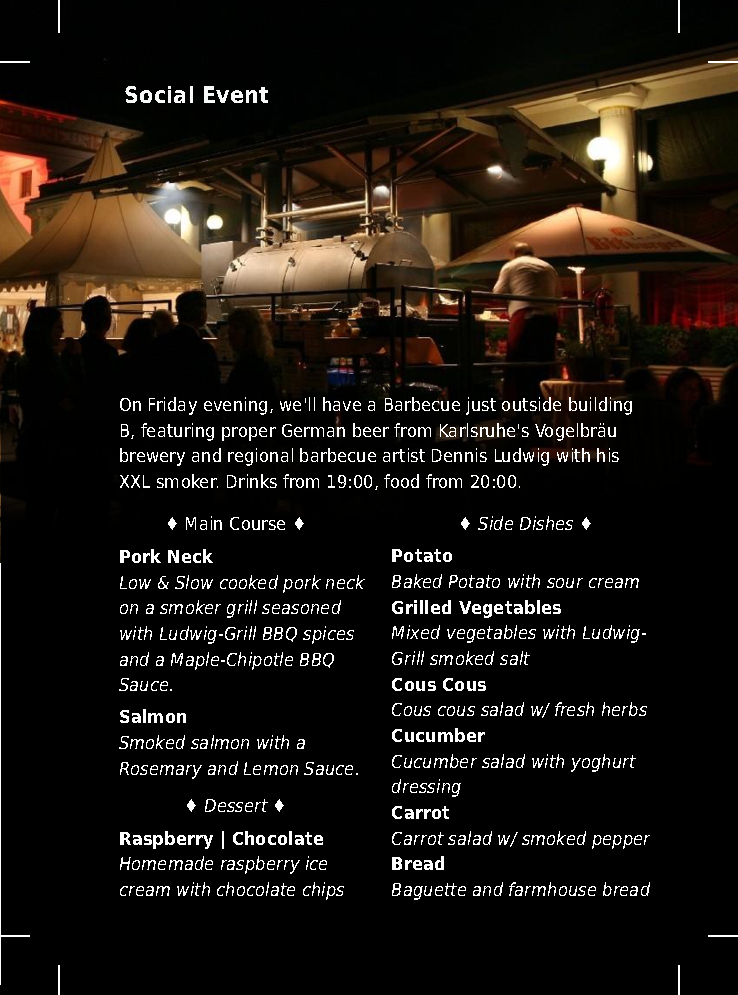
\includepdf{25-social}
\cropmarkswallpaper

\newpage
\ifthispageodd{\ThisCenterWallPaper{1.0}{generic_saturday_r}}{\ThisCenterWallPaper{1.0}{generic_saturday_l}}
\section*{Saturday}
\label{saturday}

\definecolor{geocodinggray}{gray}{.95}

\newcommand{\geocodingtalk}[2]{%
\textbf{#1} \newline\raggedright \emph{#2}%
\vspace*{0.4em}}
\renewcommand{\arraystretch}{1.4}
%\setlength{\extrarowheight}{1pt}

\begin{longtabu}{lZ{2.93cm}Z{2.93cm}}
% \begin{tabular}{p{1cm}p{3cm}p{3cm}}
% \begin{longtabu}{XX[4L]L{3cm}}
% \toprule
& \multicolumn{1}{c}{\cellcolor{b} Building B}
& \multicolumn{1}{c}{\cellcolor{a} Building A} \tabularnewline
\endhead
% \midrule
\rowcolor{commongray}
09:00 & \multicolumn{2}{C{6.27cm}}{%
\parbox[c]{14pt}{%

\includegraphics[height=10pt]{cafe}%
}
Start the day with a cup of coffee.} \tabularnewline
09:30
\talk{Versioning OSM data with GeoGit}{Victor Olaya}
\talk{Identifying  Ele-\newline
ments at Flood Risk with VGI}{João Porto de Albuquerque}
\coffeespace
\tabularnewline
% \midrule
10:00
\talk{Imposm}{Oliver Tonnhofer}
\talk{SardSOS}{Francesca Murtas}
\coffeespace
\tabularnewline
% \midrule
\rowcolor{commongray}
10:30 & \multicolumn{2}{C{6.27cm}}{%
\parbox[c]{14pt}{%

\includegraphics[height=10pt]{cafe}%
}
coffee break} \tabularnewline
% \midrule
11:00 
\talk{Sparse Editing}{Roland Olbricht}
\talk{Efficient Routing for Mobile}{Harald Koertge}
\coffeespace
\tabularnewline
% \midrule
11:30
\talk{JOSM}{Simon Legner}
\otherevent{Lightning Talks II}
\coffeespace
\tabularnewline
% \midrule
12:00
\talk{Wall·E}{Oliver Kaleske}
\otherevent{Lightning Talks III}
\coffeespace
\tabularnewline
% \midrule
\rowcolor{commongray}
12:30 & \multicolumn{2}{C{6.27cm}}{%
\parbox[c]{30pt}{%

\includegraphics[height=10pt]{photo} 
\includegraphics[height=10pt]{restaurant}%
} 
group photo, lunch until 14:00} \tabularnewline
\enlargethispage{2em}
% \midrule
14:00 
\talk{Introduction to libosmscout}{Tim Teulings}
\talk{OSM---World Map or Set of Local Maps?}{Kirill Bondarenko}
\coffeespace
\tabularnewline
% \midrule
14:30 
\talk{Combined In- and Outdoor Map App for Android}{Thomas Graichen}
\talk{Where Streets Have No Name}{Daniel Kastl}
\coffeespace
\tabularnewline
% \midrule
15:00 
\talk{}{}
\talk{Keynote}{Dirk Helbing}
\coffeespace
\tabularnewline
% \midrule
\rowcolor{commongray}
15:30 & \multicolumn{2}{C{6.27cm}}{%
\parbox[c]{24pt}{%

\includegraphics[height=10pt]{cafe}%
}
coffee break} \tabularnewline
% \midrule
16:00 
\talk{Wikipedia Tags in OSM}{Cristian Consonni }
\talk{Mapillary}{Yubin Kuang}
\coffeespace
\tabularnewline
% \midrule
16:30 
\talk{Data consistency in OSM}{Alfonso Crisci }
& 
% \multirow{2}{*}{%
% % \begin{minipage}[t][6cm][c]{3cm}
\cellcolor{geocodinggray}
\parbox[t][2.4cm][t]{3cm}{
% \vspace{-1cm}
\textbf{Geocoding Block} 
\newline\raggedright
\small{\emph{moderated by Sarah Hoffmann}\vspace*{0.5em}\newline
% \begin{itemize}
\geocodingtalk{Geocoding -- the missing link for OSM}{Gary Gale}
}}
% % \end{minipage}%
% }
\coffeespace
\tabularnewline
% \midrule
17:00 
\talk{Beyond the 3 "R"s}{Jerry Clough}
& 
\cellcolor{geocodinggray}
\parbox[t][1.7cm][t]{3cm}{\small
\textbf{Pelias} \newline
\emph{Randy Meech}\vspace*{0.4em}\newline
\textbf{OSM Gazetteer}\newline
\emph{Dmitry Kiselev}
}
%\coffeespace
\tabularnewline%
% \midrule
\enlargethispage{2em}%
17:30 
\talk{}{}
\otherevent{Closing}
\coffeespace
\tabularnewline
% % \midrule
% xx:x0 
% \talk{}{}
% \talk{}{}
% \tabularnewline
% \bottomrule
% \midrule
\rowcolor{commongray}
19:00 & \multicolumn{2}{C{6.27cm}}{%
\parbox[c]{14pt}{%

\includegraphics[height=10pt]{biergarten}%
}
Kühler Krug} \tabularnewline
\end{longtabu}
% \end{longtabu}


\ThisCenterWallPaper{1.0}{generic_saturday_r}
\vspace{1em}



\talkabstract{Versioning OSM data with GeoGit}%
{ecentralized versioning for OSM}%
{Victor Olaya is developer at Boundless, QGIS developer and main author of the QGIS processing framework.}%
{GeoGit is a decentralized versioning tool for geospatial data. This talk introduces GeoGit and discusses some of its OSM-specific features. These features bring the advantages of decentralized versioning to OSM and improve the management of OSM data.}

\talkabstract{Identifying Elements at Flood Risk with Volunteered Geographic Information}%
{An Approach based on OpenStreetMaps with a Case Study in Cologne}%
{}%
{The identification of elements at risk is an essential part in Hazard Risk Assessment. Especially for recurring natural hazards like floods, an updated database with information about critical elements at flood risk (e.g. schools, hospitals etc.) is fundamental to support crisis preparedness and response activities. However, acquiring and maintaining an up-to-date database with elements at risk requires both detailed local knowledge and hazard-specific constraints, being often a challenge for local communities due to lack of expertise and appropriate funding, deferred priorities and complex political determinations.
We present a new approach for leveraging the free and open-source mapping project OpenStreetMaps (OSM) to automatically identify hazard-specific elements at risk. We provide a new data model for extracting elements at flood risk from OSM and conduct a case study in the city of Cologne, Germany to validate our approach. Our results show that the identification of elements at flood risk with citizen-generated geodata is a suitable and cost-effective alternative for supporting local government and communities in risk assessment and emergency planning. Furthermore, the use of OSM may engage citizens in risk preparedness and risk reduction activities and thus increase risk awareness of local communities, closing the gap between citizens and governmental bodies.}

\talkabstract{Imposm}%
{The other PostGIS import tool}%
{Oliver Tonnhofer is developer of Imposm and MapProxy and co-founder of Omniscale.}%
{Imposm is an open source tool that imports OpenStreetMap data into PostGIS databases.

Imposm is fast and flexible. It supports custom database schema and can generalize complex geometries for efficient rendering.
The presentation will show you how Imposm works and in which ways it differs from osm2pgsql. You will also learn about the status of the upcoming Imposm 3 release, which will feature diff support and performance improvements.}

\talkabstract{SardSOS. More than a map}%
{An emergency call. When mappers go united}%
{Francesca Murtas is interaction designer. Mapping is a state of mind.}%
{I would like to share and talk about my experience with the free map SardSOS that I've created while confronting with the devastating floods which damaged my Island, Sardinia in November 2013(http://sardsos.crowdmap.com/). I've built an open crowdmap on the Ushahidi platform which it was based on OpenStreetMap, crowd-data and volunteer's collaboration, and mapping. The map has been visited by nearly 14.000 people in the first week, used all around the island and it has been used as a trigger, with success, for theOSM community to obtain an open license for the geo-data from the Sardinian Government. It pushed the italian mainstream media to talk about OSM and inspired other Regions/Public Administrations towards open their data and look at OSM with interest, finally seeing its opportunities. I also have done an independent, online research, after the emergency, to check the use and the perception of people of OpenStreetMap and mapping for emergencies. I
would like also to share at the SOTM  the results of the open survey done for this research. My experience, is the proof of the power of OSM, even if I'm a mapper since just one year the power of the platform and the community is just incredible.}

\talkabstract{Sparse Editing}%
{Editing large scale objects}%
{Roland Olbricht is the developer of the Overpass API.}%
{While OpenStreetMap has an impressive data quality on small scale objects, large scale objects are often only mapped in low quality. One example is the often discussed subject of mapping public transport services, and indeed these are far from complete or consistent.

The deeper reason for this is that editing large scale objects is exceptionally hard: This results from the fact that the larger an object is, the more spatial dependencies it is involved in. For example, a public transport relation can be damaged by each and every roundabout or lane mapping attempt.

In this talk we will analyse which typical kinds of dependencies exist and discuss various approaches like route suggestion by involving a route engine or mapping on a filtered subset of data. As a hands-on example it is shown how to efficiently recover a lost name tag on the river Rhine by editing an area of more than a hundred kilometers extent in JOSM.}

\talkabstract{Developing efficient routing algorithms for mobile systems}%
{Focussing on OSM and comparing against routing with professional data}%
{Harald Koertge founded his first company developing navigation systems in 1997 for PalmOS devices. Since that time, he has developed and designed multiple generations of map data models, routing engines, etc. for commercial and OSM data.}%
{As OSM is gaining more traction for usage in navigation and routing for mobile devices and applications, it’s important to understand the differences between commercial map data and OSM data, particularly for effective route calculations. Following a brief history of routing engines that were primary developed for high performance usage on mobile devices, I will share what and where the challenges are in OSM versus commercial/professional data, from the perspective of having been entrenched in both worlds for many years.}

\talkabstract{JOSM}%
{Current development and data validation using MapCSS}%
{Simon Legner has been JOSM developer since 2011, OSM mapper since 2008 and is computer scientist.}%
{JOSM is a Java-based offline editor for OpenStreetMap, which has been around since 2005.

This talk will provide insights in the current development. Emphasis will be on the usage of MapCSS for data validation which has been developed in the recent months.}

\talkabstract{Wall·E}%
{an OpenStreetMap robot}%
{Oliver Kaleske is physicist, working in software development and OSM contributor since 2010.}%
{Wall·E is a maintenance robot I have been operating in OSM-DE since the end of 2012. The edits performed range from simple tasks such as the reduction of repeatedly referenced nodes in
ways to relatively sophisticated corrections in addr:* tags. Compared to other robots, Wall·E still has a relatively low total edit count (roughly 30k by early 2014), but this also
reflects the rather conservative editing strategy employed, which includes several precautions to avoid misfixes.

The talk will cover some of the technical aspects (filtering patterns, tools involved, safety measures) as well as the robot's history starting from xybot, an earlier OSM robot which served as
a model for many of Wall·E's functions, and some remarks on the role of robots within the social system of OSM.}

\talkabstract{Introduction to libosmscout}%
{A C++ library for offline map rendering and routing}%
{Tim Teulings has been a open source and professional software developer for more than 25 years (now 43 years old). He developed a number of open source products over the year, most with a small user base. He has been working on libosmscout since around summer 2009 with an increasing user base and even some code contributions.}%
{Libosmscout is a C++ library for offline map rendering, location look up and routing. It targets mobile devices and desktop. It is highly customizable.
The talk introduces you to the project by showing potential use cases, presenting main features, giving a few simple code examples and some technical background. Discussion is expected and encouraged.}


\talkabstract{OSM: world map or set of local maps?}%
{Pecularities of national mapping}%
{Kirill Bondarenko is OSM editor since 2009. His primary interest is usage of OSM data in navigation software. He also maintains some validatation tools for the Russian community.}%
{Each country has peculiarities, and osm data is no exception. It becomes a big problem, if you need osm-based map of the world, e.g. routable map for PNA.

I will tell about local mapping rules and techniques, mainly about Russia in comparison with Europe. Tagging of common objects, address schemes, road classification, etc.}


\talkabstract{A Combined In- and Outdoor Map Application for Android}%
{A seamless in- and outdoor map viewer for OpenStreetMap data and its implementation}%
{Thomas Graichen studied information engineering at the Technische Universität Chemnitz. He is currently member of the scientific staff of the Chair for Circuit and System Design, interested in hiking, biking and therefore in OSM outdoor maps, too.}%
{Although the OSM community has realized several indoor projects, an Android application for viewing indoor maps remains unavailable. As part of an electric mobility project, the group at TU Chemnitz has developed an application that fills this gap.

The concept and an overview of the chosen implementation shall be presented here. The talk will focus in particular on the usage of the mapsforge library, which is widely used for creating outdoor maps, and how it was applied to draw indoor maps. The indoor data itself is described with the scheme proposed by Marcus Goetz (http://wiki.openstreetmap.org/wiki/IndoorOSM).

Furthermore future developments and possible usage scenarios for this map application are presented.}


\talkabstract{Where the Streets have no Name}%
{Mapping in Japan}%
{Daniel Kastl is geographer, mapper, software developer, open source and open data advocate. He was born in Germany but is currently living in Japan.}%
{From a European or North American perspective many things seem to be clear, but what you take as granted in a "Western" country is likely to be different somewhere else.
This talk gives an example, how a street-based address schema can become a real headache in countries which don't know street names.}

\talkabstract{Keynote: How to Create a Better World}%
{Planetary Nervous System, Global Participatory Platform, Social Information Technologies: How to Create a Better World}%
{Dirk Helbing is Professor of Sociology, in particular of Modeling and Simulation, and member of the Computer Science Department at ETH Zurich. He earned a PhD in physics and was Managing Director of the Institute of Transport and Economics at Dresden University of Technology in Germany. He is internationally known for his work on pedestrian crowds, vehicle traffic, and agent-based models of social systems. Furthermore, he coordinates the FuturICT Initiative (http://www.futurict.eu<http://www.futurict.eu/>), which focuses on the understanding of techno-socioeconomic systems, using Smart Data. His work is documented by hundreds of scientific articles, keynote lectures and media reports worldwide. 

Helbing is elected member of the World Economic Forum’s Global Agenda Council on Complex Systems and of the prestigious German Academy of Sciences “Leopoldina”. He is also Chairman of the Physics of Socio-Economic Systems Division of the German Physical Society and co-founder of ETH Zurich’s Risk Center. In 2013, he became a board member of the Global Brain Institute in Brussels, and in 2014 he received a honorary PhD from the TU Delft.}%
{It probably started with Linux, then came Wikipedia and Open Street Map. Crowd-sourced information systems
are central for the Digital Society to thrive. So, what's next? I will introduce a number of concepts such as
the Planetary Nervous System, Global Participatory Platform, Interactive Virtual Worlds, User-Controlled
Information Filters and Reputation Systems, and the Digital Data Purse. I will also introduce ideas such as the Social Mirror, Intercultural Adapter, the Social Protector and Social Money as tools to create a better world. These can help us to avoid systemic instabilities, market failures, tragedies of the commons, and exploitation, and to create the framework for a Participatory Market Society, where everyone can be better off.}


\talkabstract{Creating a bridge between OpenSteetMap and Wikipedia: Wikipedia-tags-in-OSM}%
{A tool to add Wikipedia tags in OSM and coordinates in Wikipedia}%
{Cristian Consonni is researcher at the "Digital Commons Lab" unit of the Fondazione Bruno Kessler (FBK), in Trento, Italy, Wikimedia Italia's vicepresident and Wikipedian, free software activist, physicist and storyteller.}%
{When you visit a Wikipedia article for a monument or a place (e.g. the Colosseum) you can find a link which will display the same object highlighted on OpenStreetMap: this tool is called WIWOSM and it was created by German mapper and Wikipedian Kolossos. It works using the "Wikipedia" tags, i.e. wikipedia=language:article, added by volunteers
in OSM.

This presentation introduces a new tool called Wikipedia-tags-in-OSM (WTOSM): a script producing a set of web pages that makes easier to add the "Wikipedia" tags in OSM using JOSM "remote control" feature, and, at the same time makes easy adding coordinates in Wikipedia articles using the {{Coord}} template and OAuth authentication. This tool has been developed by user Groppo, with a great involvement by
the Italian OSM and Wikipedia communities.

In this presentation I will present WTOSM, which is available online at http://bit.ly/wikipedia-tags-in-OSM, and its features and how it
can be used also to map places when the only information available is the Wikipedia article abstract, using Nuts4Nuts (presented at SotM13,
see http://bit.ly/presentation-Nuts4Nuts-SOTM). This project is realeased as free software (GPLv3) and its source code is available on
github.

We believe that this tool can help the OpenStreetMap community to discover new objects to map from Wikipedia pages and also it can
create a bridge among the two projects.}

\talkabstract{Data consistency in OpenStreetMap}%
{Monitoring consistency using spatial features and tag semantics}%
{Alfonso Crisci is native biometerologist/geostatistician going to OSM-ollywood with some crazy ideas.}%
{Monitoring consistency and reliability of maps is an important task when Volunteered Geographic Information (VGI) is involved and OpenStreetMap provides a good testing ground to develop operative methodologies that can be used as a web application. Two questions about data consistency are considered: for any given region (I) Is the level of spatial features density at a given scale enough for a suitable geographical description? (II) Is the semantics of the features (described by keys and tags) consistent and comprehensive?

This talk presents preliminary results from work done by Alfonso Crisci (IBIMET-CNR), Maurizio Napolitano (FBK-Trento), Francesca De Chiara (FBK-Trento), Valentina Grasso (IBIMET-CNR, LaMMA Consortium), and Cristian Consonni (FBK-Trento).}

\talkabstract{Beyond the 3 "R"s}%
{The challenges of using OpenStreetMap data for analysis}%
{Jerry Clough has been interested in maps since the age of 4. He has a professional background in scientific research (Genetics, Computer Science) and business consultancy, and is an enthusiastic amateur naturalist. OSM forms a natural nexus between these diverse interests. }%
{Most uses of OSM data fall into 3 categories, the 3 "R"s: Rendering (cartography), Routing, and 'Rummaging' (search, geolocation). However, the large and diverse sets of data within OSM also have considerable, and under-appreciated potential for answering analytical questions.

The patchiness and lack of completeness of OSM data significantly hinders its use for analysis.  But there are other aspects of the data which don't help either.

Examples of how OSM data can be used for analysis will be presented to demonstrate both the potential and the underlying issues.

Analysis places different demands on how data is mapped in OSM: a focus on using specific subsets of the data will highlight inconsistencies, and identify missing information. Furthermore it is often the case that data that is notionally derivable from OSM is not so in practice. 

Making OSM data usable for analytics tests and stresses how the data are mapped in ways which are quite different from the typical uses. Therefore particular analysis problems can help enrich and extend how and what we map.}

\newpage\ClearWallPaper

\includepdf[angle=270]{36-karte-krug}
\cropmarkswallpaper

\newpage
\ThisCenterWallPaper{1.0}{37-saturday-kuehler-krug}
\thispagestyle{empty}
\section*{Saturday Evening}

We have reserved about 100 seats at the \textbf{Kühler Krug} brewery
and biergarten pictured below, for Saturday starting 19:00. At
2.5\,km from Europaplatz (and less than 2\,km from Hotel Rio) it is
still a walkable distance away but you can also take tram No 6
from Mathystraße (direction ``Daxlanden''---don't get confused if
other sources say that Kühler Krug is served by tram No 5, this is
a temporary change). See also the map on the opposite page, or
the marker on the folded conference map.
\cropmarkswallpaper

\ClearWallPaper
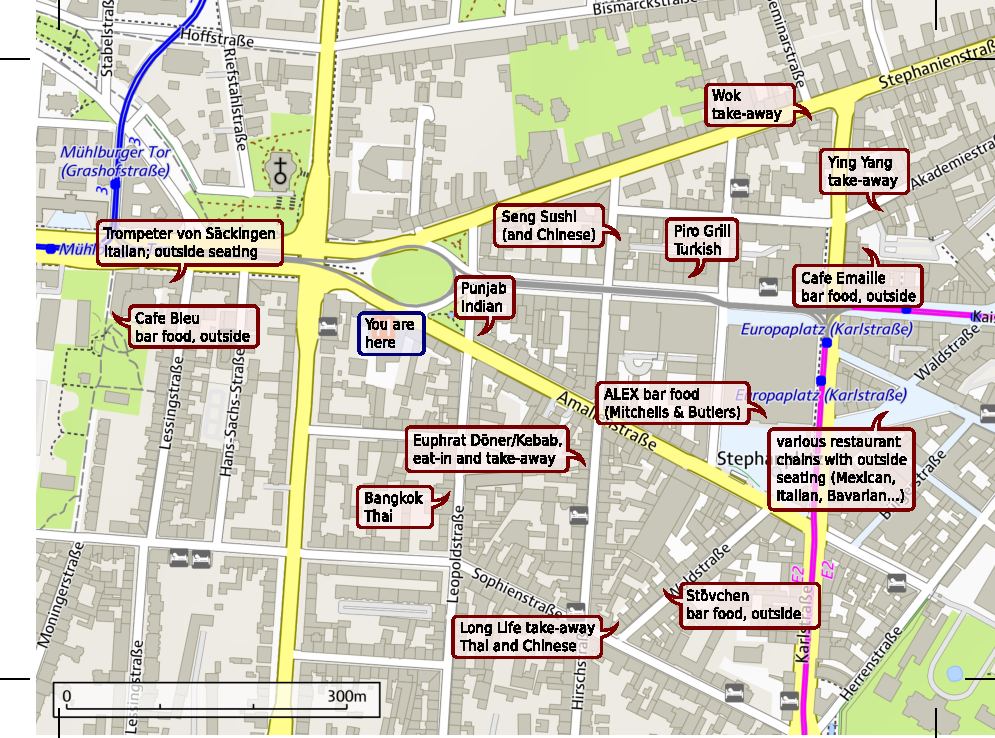
\includepdf[angle=270]{38-karte-amalien}
\cropmarkswallpaper

\newpage
\ThisCenterWallPaper{1.0}{sunday/info-hackday-background}
\thispagestyle{empty}
\section*{Sunday -- Hack Day and Workshops}

We are changing the venue on Sunday, away from the green of
the campus to the somewhat smaller inner-city university
location in Amalienstraße. Here, 
four workshops of about
one hour each will take place during the day (starting at 10h,
11h, 14h, and 15h), and there will be ample room for
hacking on your favourite OSM project. If you are more of an
outdoor type, join the excursion to a nearby nature reserve
starting at 8:00!

Hot and cold beverages are provided. At lunch, 
grab a Kebab next door, go for pizza, or sit outside at
the vibrant Ludwigsplatz down the road (see map). There's also an ice cream parlour just outside the
building, or you could order pizza from Kai's (www.kais-pizza.de).
\cropmarkswallpaper


\abstractwithspeaker{8:00}{Amalienstraße}{Jerry Clough}{Nature Mapping}%
{Sunday Morning Excursion}%
{Jerry Clough has been interested in maps since the age of four. He has a professional background in scientific research (Genetics, Computer Science) and business consultancy, and is an enthusiastic amateur naturalist. OSM forms a natural nexus between these diverse interests. }%
{This is an opportunity for interested mappers to work together in the
field to discuss, agree and document how to map and tag a range of
aspects of the natural environment. We will choose a suitable location
that offers different kinds of vegetation and habitats within 45 minutes
traveling time from the hack day location, and aim to be there by 9:00.
We will return to other hacking activities by lunch time. Follow
@SK53onOSM on Twitter for updates and last-minute changes.}

\abstractwithspeaker{10:00}{Amalienstraße}{Jochen Topf}{Osmium to the Rescue}%
{Solving OSM Problems with Osmium}%
{Jochen has been an active OSM contributor and developer of OSM software since 2006. He is co-author of a book about OSM (http://www.openstreetmap.info). He has turned his OSM hobby into a business developing software and as consultant on all things OSM and geo. More at http://jochentopf.com/ . }%
{Osmium is a highly flexible and performant C++ library for working with OpenStreetMap data. Built on top of this library are a command line tool and a Node.JS module. This suite of software can be used for many tasks, from keeping history planets current, to creating statistics, to converting OSM data in many different GIS formats. This workshop presents several typical problems from the OpenStreetMap world and shows how they can be solved using the Osmium library, the Osmium command line tool, or the Node.JS module. 

You can find more about Osmium and related software at http://osmcode.org/. }

\abstractwithspeaker{11:00}{Amalienstraße}{Roland Olbricht}{Overpass API v0.7.50}%
{The Temporal Dimension}%
{Roland Olbricht is the developer of Overpass API. }%
{With OpenStreetMap getting more mature, it becomes more important to track changes. But to track changes is difficult for various reasons: Changeset comments can be misleading, destruction may be hidden in innocent looking changes, and the sheer amount of data prohibits a complete manual review. For that reason Overpass API provides, from version 0.7.50 on, the complete history since the license change. 

In this workshop we'll demonstrate the commands to access that data: getting data as it was at any chosen point in time; getting even a changefile of what has changed between two points in time. This is complemented by a feature to print the full geometry of a way or relation without referring explicitly to its nodes. We explain how these features allow building powerful client JavaScript only websites that can track changes with arbitrary search criteria. We will discuss what remains to be done to build a complete and logically consistent revert tool based on Overpass API v0.7.50. }


\abstractwithspeaker{14:00}{Amalienstraße}{Andy Allan}{OpenStreetMap Carto}%
{The State of the Style Sheets---One Year On}%
{Andy is a freelance digital cartographer and open-source geospatial developer. He has been creating maps from OSM data since 2007 and started the OpenStreetMap Carto project in November 2012. }%
{ In this workshop we will review our progress over the last 12 months, lay out the future roadmap and look at some of the interesting projects that have used OpenStreetMap Carto as a foundation. We will also find the time to discuss individual design choices and issues, and methods to fix them.
}

\abstractwithspeaker{15:00}{Amalienstraße}{Martijn van Exel}{MapRoulette Next Generation}%
{User Defined Challenges}%
{Martijn's bond with OpenStreetMap dates back to 2007, when he attended his first mapping party in Amsterdam. He was hooked and became a community leader in the Netherlands. He continued this role when he moved to the United States in 2011. He has been serving on the United States Chapter board since then - the last two years as president. Martijn works at Telenav, a global provider of personal navigation software, as an OSM expert. }%
{TBD
}%

\newpage
(for your notes)

\newpage
(for your notes)

\newpage
\section*{Imprint}
\label{imprint}

\begin{raggedright}
State of the Map Europe 2014 is jointly organised by FOSSGIS
e.V. and the Karlsruhe University of Applied Sciences
(Hochschule Karlsruhe).

\vspace{0.5em}
 \begin{minipage}[htbp]{0.47\textwidth}
	
\includegraphics[width=\linewidth]{FOSSGIS}
\end{minipage}
\hfill
\begin{minipage}[hbtp]{0.47\textwidth}

\includegraphics[width=\linewidth]{hochschule-logo}
\end{minipage}

\vspace{1.6em}
\noindent responsible for the content:\\
FOSSGIS e.V.\\
Theodor-Echtermeyer-Straße 15\\
14469 Potsdam

\vspace{1em}
\noindent This booklet has been prepared by Michael Reichert and Frederik
Ramm using Open Source Software. Photos by Ludwig Grill and 
Christine Karch.

\vspace{0.5em}

\noindent All maps have been made by Holger Schöner based on Open\-Street\-Map
data, copyright OSM contributors, licensed Open Database License 1.0.

\vspace{0.5em}
\noindent The icons used in the tables are licensed CC-0 by SJJB Management. Grass 
clipart Public Domain by cyberscooty via openclipart.org.


\vspace{1em}
\noindent \begin{minipage}[htbp]{0.2\textwidth}
\noindent
\includegraphics[width=\linewidth]{cc-by-sa}
\end{minipage}
\hfill
\begin{minipage}[hbtp]{0.74\textwidth}
The whole of this booklet may be re-used under the Creative
Commons Attribution Share-Alike 3.0 license.
\end{minipage}
\end{raggedright}


\ClearWallPaper

\includepdf{U4-sponsoren}
\cropmarkswallpaper


\end{document}
